%\documentclass[journal,10pt]{article}
\documentclass[journal,10pt]{IEEEtran}
\usepackage{hyperref}
\usepackage{todonotes}
\usepackage{amssymb}
\usepackage{amsmath}
\usepackage{mathtools}
\usepackage{graphicx}
\usepackage{soul} 

\newcommand{\subtask}[1]{\begin{quote}\textbf{#1}\end{quote}}
\newcommand{\hod}{h}
\newcommand{\moh}{m}
\newcommand{\dow}{d}
\newcommand{\dom}{d_m}
\newcommand{\wom}{w_m}
\newcommand{\woy}{w_y}
\newcommand{\yyy}{a}

\newcommand{\IN}{\mathbb{N}}
\newcommand{\defeq}{\coloneqq}

\author{Jan Lippert \(<\)\href{mailto:ljan@mail.upb.de}{ljan@mail.upb.de}\(>\)}
\date{\today}

\begin{document}

\title{Predicting Parking Space Availability in Paderborn}
\maketitle

\begin{abstract}
The Parking Prediction system Paderborn is available at \url{http://pppb.herokuapp.com/}. It was written in Play! Scala and uses the \href{smile}{haifengl.github.io/smile/} library. the system regularly predicts the number of available parking spaces for the ``Libori-Galerie'' 15 minutes in advance.
\end{abstract}

\tableofcontents
\begin{itemize}
  \item Topic introduction
  \begin{itemize}
    \item \st{What question does your work answer}
    \item \st{What related work does exist}
    \item Why did you choose your topic
  \end{itemize}
  \item Methodology choice
  \begin{itemize}
    \item Introduction of chosen methodology\todo{extend section \ref{sec:training_model} by introducting regression trees}
    \item \st{Motivation behind choice}
    \item Discussion of possible problems with data or methodology
    \item Comparison between methodologies, if applicable
    \begin{itemize}
      \item GradientBoost may lead to better results
      \item Add comparison and ``why''
    \end{itemize}
  \end{itemize}
  \item Verification
  \begin{itemize}
  	\item \textbf{TODO. Needs a lot of work!}
  \end{itemize}
  \item Run-time technology
  \begin{itemize}
    \item \st{Introduction of run-time system}
    \item \st{Technology choices and motivation}
    \item Discussion of possible problems with setting up run-time system
  \end{itemize}
  \item Results
  \begin{itemize}
    \item Result of your work (hypothesis statement)
    \item Discussion of prpossible future work
    \item Reflection against existing literature
  \end{itemize}
  \item Reflection
  \begin{itemize}
    \item What did you learn
  \end{itemize}
\end{itemize}






\section{Introduction}

\subsection{What question does your work answer}
In urban areas, space and as such parking space is limited. Car owners often have to drive around to available parking spots. This leads to an unnecessary waste of time and additional air pollution. 

According to multiple studies, the availability of parking data reduces the search time for a parking spot \cite{Asakura1994}\cite{Caicedo2010228}. However, most systems only provide the current number free parking spots. In rush hours, this information can quickly get outdated and lead to driving around to find available parking spaces.

In Paderborn the situation is similar: live-data is available but no prediction. The goal of this project is exactly that. Because of the limitation outlined in \ref{sec:challenges}, data-crawling and future predictions will focus on the covered car park ``Libori-Galerie''. This car park is also the most interesting as it is directly connected to a local shopping center. 




\subsection{Related Work}
\cite{parkendd} is a similar project which used the collected data to predict parking space availability. This project focussed on the car park ``Centrum Galerie''. \cite{parkendd} used the following features: week of year, day of week, time of day, sunday openings and the number of workdays until the next public holiday. Sunday openings are used as in Germany, shops are normally closed on Sundays. Sunday openings therefore influence how many people go to the shopping center and therefore the availability of parking space. In \cite{parkendd}, different algorithms are compared and the predictions are evaluated.

\cite{Rajabioun2013} propose parking guiding and
information system which also includes the prediction of available parking space. The proposed algorithm uses a probabilistic model based on historical data. Among others, the used features also include time of day and day of week. At last, \cite{Rajabioun2013} estimates the mean-error on predictions. They mention that predictions for 10 minutes in the future lead to a 1.2\% error on average while predictions for 40 minutes in the future lead to a 2.8\% error on average.

\cite{Zheng2015} compared three different feature sets and three different machine learning algortihms -- regression tree, neural network, and support vector regression -- with respect to their performance. Based on data from the cities of Melbourne and San Francisco they conclude that the regression tree provides the best predictions when used with a feature set containing day of week and time of day.  


\section{Methodology choice}

Since this work is inspired by \cite{parkendd}, a RegressionTree model was chosen as machine learning method. To keep the complexity of the application in check, the model was kept simple: the data consisted only of timestamped availability data.

\subsection{Data Sources}\label{data sources}
The main data source is the actual parking data which is available online. In addition there are other possible features that may influence parking space availability. Since taking all features into account is not possible, this project will solely focus on the parking data in relation to time. 

\paragraph{Parking Usage Live Data}
The homepage of the ASP Paderborn\footnote{City-Managed service for waste management, city cleaning, and parking.} lists the city managed parking areas and the number of currently free parking spots. 
The data is available on \url{https://www.paderborn.de/microsite/asp/parken_in_der_city/freie_Parkplaetze_neu.php}. A more minimal website is available at \url{https://www4.paderborn.de/ParkInfoASP/default.aspx}. 

The website displays 4 attributes: name, type, capacity, and available spots\footnote{respectively: Parkstätte, --, Anzahl, Frei}. After crawling, the parking information will be annotated with the crawling time. The latter will be split into multiple attributes which will be used in the prediction: hour of day \(\hod\), minute of hour \(\moh\), day of week \(\dow\), day of month \(\dom\), week of month \(\wom\), week of year \(\woy\), and \(\yyy\)\footnote{the year is included as a way to keep samples unique in case the project runs more than 1 year.}.

The number of available parking spaces is be called \(y\). With the features defined before, the training data will be a set of tuples of the form  
\[
(\hod, \moh, \dow, \dom, \wom, \woy, \yyy, y)\text{.}
\]

\paragraph{Other data-sources}
It was also considered to enrich the data set by adding event and holiday data as both could influence the parking situation near the city center. In some cases, these events take place on one of the parking areas or directly besides them. However, as most of the big events do not happen while the course ``Practical Project in Machine Learning'' takes place, they will not considered further.

\begin{figure}
  \centering
  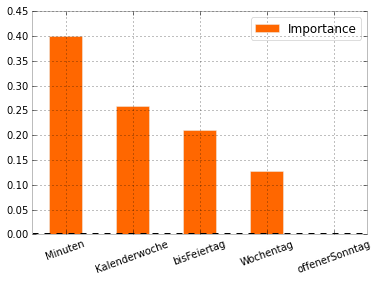
\includegraphics[scale=0.5]{parkendd-Feature-Importance.png}
  \caption{Importance of Features (ParkenDD)}
  \label{fig:parkendd_features}
\end{figure}

Public holidays like Christmas and Easter may also influence the availability of parking space. \cite{parkendd} modeled this in the feature ``bisFeiertag'', i.e. working days until public holiday. In figure \ref{fig:parkendd_features}, the relevance of the different features used by \cite{parkendd} is displayed\footnote{respectively: minutes, week of year, working days until public holiday, day of week, Sunday openings}. 

The feature was relatively important in the evaluation done by \cite{parkendd}. Nonetheless, it will not be included as the next public holiday is Christi Himmelfahrt on 25th May 2017. Therefore there would be no possibility of verifying the importance of this feature in time.

Weather data was also considered as an additional source of information because, e.g., more people may decide to take the car when it's raining. Although such data is available online in machine-readable formats, it will not be considered to keep the model simple.

\subsection{Hypothesis \& Training Method}\label{sec:training_model}

It is assumed, that the available parking space is dependent on time, i.e. there exists a function \(f\) such that 
\[
f(\hod, \moh, \dow, \dom, \wom, \woy, \yyy) = y\text{.}
\]

As mentioned in previous sections, the idea to predict available parking space was inspired by other projects. \cite{parkendd} was using a RegressionTree model with great success, so I picked this model.

To keep the scope of this project small, multiple data sources will be ignored. For this project, it is assumed that the number of available parking spots solely depends on time. As described in \ref{data sources}, this obviously is a very simplified model. However, as shown by \cite{parkendd}, such a simple model may be enough. 

%The greatest challenge in this project is to collect enough training data to make meaningful predictions. All data needs to be extracted from ASP's website. Changes to the website and non-availability of the service may prove problematic. In the beginning of February, the ASP parking guiding system was dysfunctional and did not show useful data for one week. 

\section{Verification}
\begin{table}
  \centering
  \caption{Evaluation per day of year}
  \label{tab:eval_doy}
  \begin{tabular}{rrrr}
  \(date\) & \(n\) & \(MAE\) & \(\sigma\) \\
  \hline 
  01.03.   &  103  &   26.14 &  36.35 \\
  02.03.   &  185  &   23.64 &  29.54 \\
  03.03.   &  286  &   21.24 &  24.80 \\
  04.03.   &  521  &   39.06 &  36.61 \\
  05.03.   & 1091  &   67.32 &  47.67 \\
  06.03.   & 1082  &   51.28 &  45.73 \\
  07.03.   &  925  &  204.89 & 127.97 \\
  08.03.   &  969  &  186.90 & 172.56 \\
  09.03.   & 1050  &   20.70 &  28.86 \\
  10.03.   & 1085  &   25.24 &  27.12 \\
  11.03.   &  586  &   30.31 &  40.46 \\
  \end{tabular}
\end{table}


The functionality of the system will be verified by doing regular predictions and comparing these to the actual 
parking situation later. Similar to the crawling implementation, the web application will generate a new prediction 
``15 minutes into the future''. These predictions will be saved in a database. 

To measure the error, we will use the mean absolute error 
\[
MAE \defeq mean(|y_i^∗ - y_i|)\text{,}
\]
where \(y_i^∗\) denotes the predicted value and \(y_i\) denotes the actual, crawled value. Table \ref{tab:eval_doy} lists the evaluation results fetched on 11.03.2017 around 6pm. 

The evaluations show that the predictions got worse on the 4th and are especially bad on the 7th and 8th March. The cause for this was some experimentation with the training method and the model.

On the 4th, the training method was adapted. Instead of generating 10 GradientBoostTrees with shrinkage values from 
\(0.1\) to \(1\) (step width \(0.1\)), only 4 GradientBoostTrees with fixed shrinkage values of (\(0.001\), \(0.01\), 
\(0.1\), and \(1\) were generated. According to \href{http://haifengl.github.io/smile/index.html#gbm}{the documentation of GradientBoost}, 
the shrinkage parameter controls the learning rate; it was assumed that picking a set of four very different values
would sufficient for good predictions.

On the 7th, the model attributes ``week of month'' and ``week of year'' were removed. All Learning models compute the 
so-called importances of the attributes used for learning. According to the importances determined in previous 
predictions, the aforementioned attributes were not important. Also, from this day on the attributes were normalized 
when training the model. This was not necessary but I wanted to try it out anyway.

As one can see in Table \ref{tab:eval_doy} both changes did not improve the model but instead made predictions worse. Therefore the changes were rolled back on the 9th. After this was done, the prediction accuracy increased again. 
Figures \ref{fig:actual} and \ref{fig:predictions} display the actual availability respectively the predicted 
availability of parking spaces over the last 48 hours. As one can see, the tendency of the predictions is quite good. However, the predictions tend to overshoot and ``wiggle around''. When presenting the intermediate results in class, it was suggested to dampen the predictions. 

\begin{figure}
  \centering
  \caption{Crawled parking space availability}
  \label{fig:actual}
  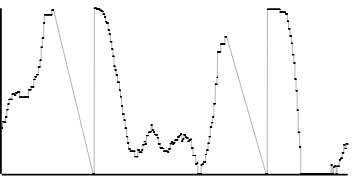
\includegraphics[scale=0.5]{fig_actual}
\end{figure}

\begin{figure}
  \centering
  \caption{Predicted parking space availability}
  \label{fig:predictions}
  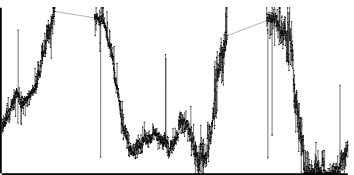
\includegraphics[scale=0.5]{fig_predictions}
\end{figure}


%\section{Results}
%\subsection{Result of your work (hypothesis statement)}
%\subsection{Discussion of possible future work}
%\subsection{Reflection against existing literature}



\section{Run-time technology}

It was chosen to develop the web application in Scala using the Play! framework, mainly because of familiarity with the language and its usage in machine learning applications. It is also used in  

\subsection{Architecture}\label{sec:architecture}
One important part in the choice of technology was the separation of the different concerns in the applications. There are multiple parts that play together: crawling, preprocessing, training, prediction, and finally evaluation. 

Crawling has to be done on a regular basis. Therefore the chosen framework needs to support regular execution of jobs. When new entries are crawled, they are cleaned via the preprocessing module and inserted in the database. Since it may be necessary to update the model over time, the preprocessing module will also have a regular job that cleans existing entries by updating them to the most recent model.

\subsection{Frameworks}\label{sec:frameworks}
To implement this project, Ruby on Rails, Python and Scala were considered. I used Ruby on Rails in previous projects and development is quite fast with this framework. However, I could only find a few libraries that deal with machine learning \cite{bigml} \cite{leanpanda}. 
Another choice of language was python. Python has quite a lot pf machine learning libraries and is also used in academics. However, I do not have much previous experience with python.

My final choice was the \href{Play! framework}{https://playframework.com} with Scala. I did use this framework in previous projects and therefore was familiar with setting up background jobs and how to enable web access. Heroku also supports easy deployment for Play! applications\todo{insert links in final report}. One important factor of this choice was the type-safety of the Scala language and it's usage in machine learning and big data\todo{insert link in final report}. While the problem at hand is certainly not big data, the multitude of existing libraries helped a lot to get started\todo{add links to the libraries in final report}.

I chose to use \href{Smile}{http://haifengl.github.io/smile/index.html}, the ``Statistical Machine Intelligence and Learning Engine''. It was easy to use and documentation is quite extensive. In some cases, the API documentation even references the scientific papers the learning algorithm is based on. 


\section{Encountered Problems}\label{sec:challenges}
\subsection{Malfunction of the Parking Guidance System}
One week after the first prototype of the crawler was online, \url{https://www.paderborn.de/microsite/asp/parken_in_der_city/freie_Parkplaetze_neu.php} was non-functional. The number of available parking spaces for the ``Liborie-Galerie'' was always set to \(0\).

At the same time, many of the other parking areas were switched to ``Nicht im Parkleitsystem'' (not part of the parking guidance system). Both of these issues were caused by a malfunction of the parking guidance system. Crawling was resumed normally after the parking guidance system was fixed by the provider.

On another note, string values were not expected for the Liborie-Galerie. This caused the crawler to crash on every crawl; the crawler was then adapted to be ore resilient to unexpected values: all non-integer values for free spaces will directly be dropped.


\subsection{Heroku Free Limitations}
After collecting data for some time, I did some correlation analysis on the data. I noticed that all entries had ``\(\wom = 1\)'' despite the app being online for more than a week. Further investigation showed that the data was only available for 3 different days. 

The reason for this failure was the uninformed use of the Heroku Free package. Free dynos will sleep after 30 minutes minutes of inactivity. After this was noticed, multiple services and workarounds were investigated.

However, most of the workarounds were from before 2015. In 2015, Heroku added the requirement that free dynos need to sleep 6 hours a day. Unfortunately the most promising service -- \url{http://kaffeine.herokuapp.com/} -- is not functional anymore.

To keep the system running, a bash script was created which keeps the dyno awake by sending regular HEAD requests. Since the dyno is still required to sleep 6 hours a day, a sleeping time had be chosen. Luckily, the ``Libori-Galerie'' is closed from 2am to 8am and the dyno will rest in this period. 

Also, there were multiple problems in accessing the database The free tier only allows 20 concurrent connections to the Postgresql database. These connections were exhausted 5 minutes after the start of the application. This could be solved by configuring the application to restricting the number of database connections to 10 -- when the application was configured to use 20 connections, problems persisted.

The next limit is in the size of the database. The free tier only allows \(10000\) rows. Insert actions will be disabled after the database has had more than \(10000\) for 7 days. This challenge will be circumvented by removing old data in regular intervals.



\section{Reflection}
The most important lesson I learned was: do more regular checks of a deployed system. Many of the problems were discovered too late because ``it worked on my local machine''. All of these could have been avoided by checking the web app more regularly or setting up some service to check the system.

Another important lesson was that doing machine learning without previous experience is hard. This was my first machine learning course; learning the methods and implementing at the same time was very challenging. However, the gained experience was worth it.


\section{Addiotional todos}
\subsection{Model iterations}

Week of month was removed. was not important in training. unsurprising result
\bibliographystyle{ieeetr}  
\bibliography{report_lippert}

\end{document}
